 \documentclass{beamer}
 \usepackage{amsmath}
 \usepackage{amssymb}
 \usepackage{graphicx}
 \usepackage[polish]{babel}
 \usepackage[utf8]{inputenc}
 \usepackage{polski}
 \usetheme{Ilmenau}
 \usecolortheme{beaver}
 
 \author{Marcin Ochman}
 \title{Warcaby - projekt na PAMSI}
 \date{}
 \institute{Politechnika Wrocławska}
 \begin{document}
  \begin{frame}
		\titlepage
  \end{frame}
  
  \begin{frame}
 	\frametitle{Warcaby - zasady gry}
 	\begin{itemize}
 	   \item Gra prowadzona jest na szachownicy o wymiarze 8x8
 	   \item Figury poruszają sie po czarnych polach
 	   \item Pierwszy ruch należy do pionków szarych
 	   \item Pionki mogą poruszać się tylko o jedno pole do przodu
 	   		 	po ukosie
 	   \item Pionki mogą bić tylko przeskakując nad pionkiem 
 	   			przeciwnika i ustawiając się na pierwszym polu za 
 	   			nim, można to robić kilkukrotnie (rekurencyjnie)
 	   \item Gdy pionek dojdzie do końca planszy, staje sie matką
 	   \item Matki poruszają się po skosie do tyłu i do przodu o 
 	   			dowolną liczbę pól
 	   \item Matka bije przeciwnika przeskakując na pole za nim 
 	   			(niekoniecznie pierwsze), można to robić 
 	   			kilkukrotnie (rekurencyjnie)
 	\end{itemize}
  \end{frame}
  
  
  \begin{frame}
  	\frametitle{Algorytm Min-Max}
  	 \begin{figure}[H]
       \centering
  	   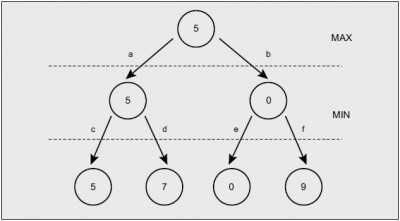
\includegraphics[width=0.7\linewidth]{./img/minmax}
  	   \caption{Idea działania algorytmu Min-Max}
  	   \label{fig:minmax}
  	 \end{figure}
  \end{frame}
  
  \begin{frame}
  	\frametitle{Wygląd gry}
  	\begin{figure}
      \centering
      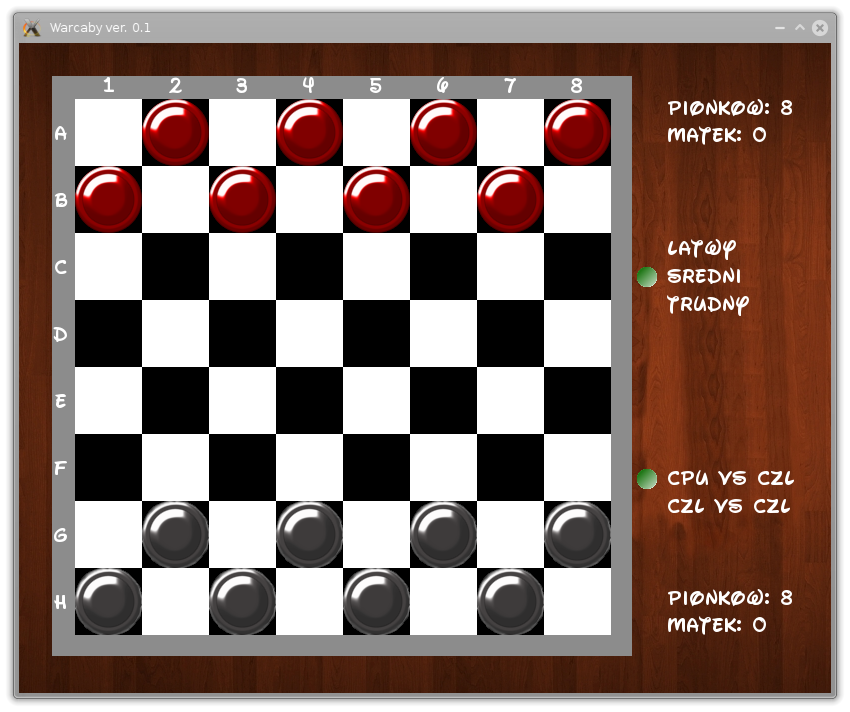
\includegraphics[width=0.7\linewidth]{./img/warcaby}
	  \caption{Zrzut ekranu z gry Warcaby}
	  \label{fig:warcaby}
	\end{figure}
  \end{frame}
  
   \begin{frame}
    	\frametitle{Lista użytych klas}
    	\begin{itemize}
    	   \item Macierz	
    	   \item PlanszaWarcaby
    	   \item Pole	
    	   \item Sciezka
    	   \item Warcaby
    	   \item WarcabyGUI	
    	   \item Wspolrzedna
    	\end{itemize}
    \end{frame}  
 \end{document}